\chapter{Conceptos básicos}
\label{chap:conceptos_basicos}

\lettrine{P}{ara} una correcta comprensión de los objetivos, tanto a corto como a largo plazo, de este trabajo, es necesario entender los conceptos básicos sobre los que se apoya esta línea de investigación.

\section{Redes neuronales}
\label{sec:redes_neuronales}
Las redes neuronales constituyen la base de la mayoría de últimos avances en el campo de la inteligencia artificial, y a pesar de la enorme diversidad en \textit{layouts} de capas, neuronas, funciones de transferencia, etc, la realidad es que el álgebra lineal y la multiplicación de matrices son parte fundamental e imprescindible para la ejecución de las mismas. \cite[Figure 3.4]{deep_learning_for_computer_architects}

A pesar de que en la \acrshort{poc} (\acrlong{poc}) expuesta más adelante en este trabajo se trabaja únicamente con redes \textit{Feed-Forward}, sería naíf pensar que solamente existen estas arquitecturas de redes neuronales. Ejemplos a destacar serían las redes convolucionales, empleadas principalmente para el procesado de imágenes, las basadas en modelos secuenciales o en transformers, que están revolucionando el mundo de la inteligencia artificial mediante modelos de procesamiento del lenguaje o de generación de imágenes, así como muchas otras como las redes GAN, o las basadas en Encoder-Decoder.

Estas arquitecturas son llamadas de redes neuronales, a pesar de que como es evidente, una neurona no puede, como tal ``ejecutar'' una convolución. Más bien, estas nuevas arquitecturas se basan en la modelación de operaciones matemáticas complejas en pasos discretos como, por ejemplo, la convolución que se menciona previamente.

\subsection{Estructura de una red neuronal feed-forward}
\label{ssec:estructura_red_neuronal_ff}
Las redes neuronales \textit{feed-forward} se componen de varias capas de neuronas que toman una o más entradas, realizan la suma de todas ellas, suman un \textit{bias}, y finalmente aplican una función de transferencia no lineal.

La capa que toma los datos de entrada se llama capa \textit{input} o de entrada, y la capa que expulsa los datos de salida es la capa \textit{output} o de salida. Las capas que realizan transformaciones intermedias se denominan capas ocultas, o \textit{hidden layers}.

En la Figura \ref{fig:dense_nn_sample}\footnote{Imagen generada con la herramienta NN-SVG, disponible en \url{https://alexlenail.me/NN-SVG}} se puede ver un diagrama de una red neuronal Feed-Forward densa. Esto es, una red neuronal en la que cada neurona de una capa está conectada con todas las neuronas de la capa a continuación. Esto se traduce en que la matriz de pesos que representa cada capa es una matriz densa, o dicho de otra manera, que no contiene pesos con valor 0.

\begin{figure}[h!]
    \centering
    \vspace*{0.5cm}
    \def\svgwidth{0.85\textwidth}
    \input{pdf_tex/dense_nn/dense_nn_svgnn.pdf_tex}
    \caption{Red neuronal densa Feed-Forward}
    \label{fig:dense_nn_sample}
\end{figure}

Por el contrario, y como se puede ver en la Figura \ref{fig:sparse_nn_sample}, existen las redes neuronales dispersas, en las que una cantidad significativa de los pesos tienen valor cero. Estas redes se pueden obtener de múltiples formas, y sus objetivos son variados, a pesar de que el principal objetivo es reducir el tamaño del modelo.

Uno de las posibles métodos para la obtención de una red neuronal dispersa (\textit{sparse}) es mediante el podado o \textit{pruning}. Este método, sorprendentemente similar al empleado por neurocirujanos durante operaciones a cerebro abierto, consiste en ir cortando de forma más o menos arbitraria (en función del algoritmo) conexiones y observando cómo varía la salida. En caso de que la salida sea correcta, se continúa en esa dirección. Para que un cambio en una red neuronal se considere inapreciable, la salida debe verse alterada de tal forma que sea indistinguible su efecto del de unos diferentes parámetros iniciales durante el entrenamiento.

De esta forma, una red neuronal dispersa puede contener alrededor de un 80\textasciitilde90\% menos de conexiones entre neuronas, representando esto un ahorro sustancial de energía en términos de acceso a memoria, relevante en sistemas miniaturizados donde cada miliwatt cuenta.

\begin{figure}[h!]
    \centering
    \vspace*{0.5cm}
    \def\svgwidth{0.85\textwidth}
    \input{pdf_tex/sparse_nn/sparse_nn_svgnn.pdf_tex}
    \caption{Red neuronal dispersa Feed-Forward}
    \label{fig:sparse_nn_sample}
\end{figure}

Esta operación de podado puede no solamente limitarse a los pesos que interconectan neuronas, sino que se puede hacer el modelo más eficiente y reducido al podar todos los pesos entrantes en una neurona, eliminando por completo dicha neurona, a la vez sus conexiones posteriores en cadena. El efecto de eliminar una neurona sin conexiones entrantes, que únicamente arroja valores constantes en cada iteración, se puede compensar ajustando el \textit{bias} del receptor que correspondía a esa neurona en las conexiones posteriores.

\subsection{Redes neuronales profundas}
\label{ssec:redes_reuronales_profundas}
El \textit{boom} de la inteligencia artificial en los últimos años viene dado en gran medida por el enorme crecimiento que ha experimentado el sector mediante técnicas de \textit{deep learning}, precisamente en estas redes neuronales profundas o \textit{deep neural networks}.

Y es que dentro de las infinitas posibilidades que nos ofrecen las ``neuronas'' tratadas anteriormente, existe la posibilidad de apilar capa sobre capa, obteniendo a cada capa extra comportamientos y patrones más complejos.
Es precisamente este comportamiento de los sistemas no lineales el que permite reproducir comportamientos exóticos al aumentar el número de neuronas y/o capas (y por tanto la complejidad) del sistema.

Tras sospechas previas de algunos investigadores como George Cybenko acerca de que una red neuronal con al menos una capa oculta es un aproximador universal, y tras demostrar dicho comportamiento para la sigmoide como función de transferencia \cite{cybenko1989approximation}, Kurt Hornik demostró en 1991 que una red neuronal de con al menos una capa oculta es siempre un aproximador universal, independientemente de la función de transferencia, siempre que esta sea no polinomial. A pesar de que una red neuronal de una sola capa oculta pueda ser un aproximador universal, se obtienen aproximaciones mucho más inteligentes y ``económicas'' computacionalmente al contar con más de una capa oculta \cite{hornik1991approximation}.



\section{Redes neuronales densas}
\label{sec:redes_reuronales_densas}
Como se comenta en la sección anterior, independientemente del número de capas de la red, sea profunda o ``convencional'', una red neuronal densa es aquella en la que para $m$ neuronas en la capa $M$, y $n$ neuronas en la capa $N$, donde la neurona $x$ de la capa $M$ se denota $M_{x}$ existe siempre una conexión de $M_{m}$ a $N_{n}$, es decir ($m\longrightarrow n$):

\begin{equation}
\forall m \in M \:\wedge\: \forall n \in N, \: m\longrightarrow n
\label{eq:dense_nn}
\end{equation}

De esta forma, para la ejecución (inferencia) de una red neuronal densa feed-forward, serán necesarias únicamente una simple multiplicación de matrices, una suma de matrices para tener en cuenta los \textit{bias}, y aplicar una función de transferencia.

Esto se puede apreciar en la Figura \ref{fig:nn_matrix_dense}\footnote{Imágenes con este estilo artístico han sido obtenidas de \url{https://ml-cheatsheet.readthedocs.io/en/latest/forwardpropagation.html}}. En ésta se puede ver la inferencia de 4 datos, correspondientes con el número de filas de entrada a las capas. Como también se puede apreciar, la anchura de cada capa se corresponde con el número de columnas de la misma. 

\begin{figure}[h!]
    \centering
    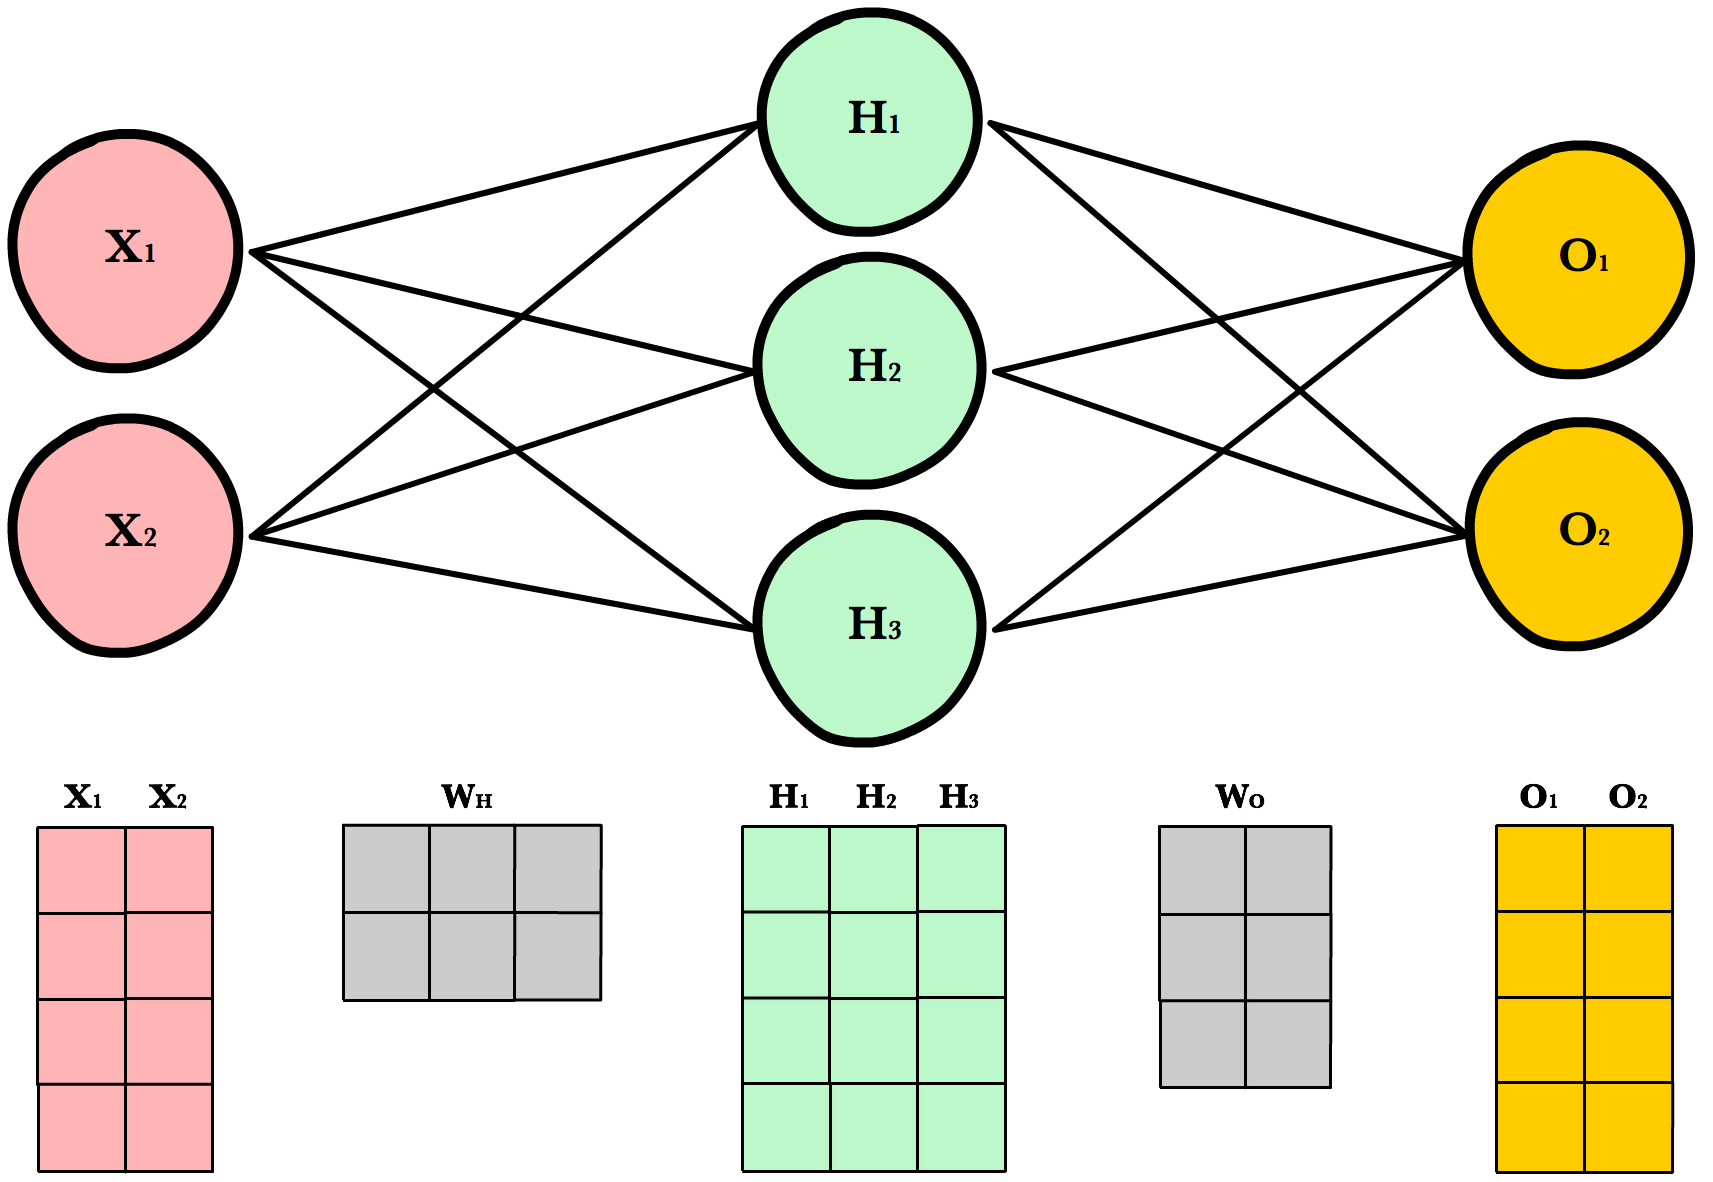
\includegraphics[width=0.85\textwidth]{img/neural_network_matrix_dense.png}
    \caption{Visualización de inferencia en redes neuronales densas}
    \label{fig:nn_matrix_dense}
\end{figure}

De esta forma, si el dato (vectorial por la naturaleza de estas redes) tiene 24 elementos, será necesaria una capa de entrada de 24 neuronas (24 columnas $x_{1} .. x_{24}$ según notación de la Figura \ref{fig:nn_matrix_dense}), y si queremos inferir sobre 1000 de estos datos, esto se puede hacer en una sola ejecución, siendo el número de columnas también de 1000.

O dicho de otra manera, sea la capa $M_{m}$ una capa completamente conexa con $m$ neuronas, a la cual se le introduce un dato $x_{m}$, donde el peso de la neurona $M_{i}$ hacia $N_{j}$ es denotado por $w_{M,i,j}$, y la función de transferencia es $\phi$, tenemos que la salida de una capa será:

\begin{equation}
    x_{N,i} = \phi\left(\sum_{j}w_{N,i,j}x_{M,j}\right)
    \label{eq:dense_nn_eq}
\end{equation}

A esta función se le puede añadir el \textit{bias} de forma explícita ($\sum\left([\dots] x_{M,j}\right) + bias_{N,i}$), o de forma implícita, siendo el \textit{bias} una conexión más, con un valor constante de 1, cuyo peso es el multiplicador que da el \textit{bias} resultante.

\section{Redes neuronales dispersas}
\label{sec:redes_reuronales_dispersas}
Las redes neuronales dispersas cuentan con una ventaja, y es el menor número de conexiones entre neuronas, o directamente el menor número de neuronas en la arquitectura. A pesar de esto, en realidad el fundamento matemático es el mismo, una simple multiplicación de matrices. Sin embargo, a pesar de ser el mismo funcionamiento base, se pueden explotar ciertas características tanto de la estructura de las matrices dispersas como de su multiplicación para obtener mejorías en el tamaño del modelo o en rendimiento, respectivamente.

\subsection{Fundamentos de matrices dispersas}
\label{ssec:fundamentos_matrices_dispersas}
Una matriz es dispersa cuando gran parte de su contenido son únicamente ceros. El cuan dispersa es una matriz se cuantifica mediante el ``grado de dispersión'' o \textit{sparsity}. Una matriz dispersa $10 \times 10$, con tres elementos diferentes de cero (\textit{non-zero elements} o directamente \textit{non-zero(es)}) será una matriz dispersa con una \textit{sparsity} del $97\%$, y una densidad del $3\% \:(=100\%-97\%)$.

\subsection{Almacenamiento de matrices dispersas}
\label{ssec:almacenamiento_matrices_dispersas}
Existen múltiples métodos para el almacenamiento de matrices dispersas en memoria, pero uno de los más sencillos de comprender, y que se usa en la \acrshort{poc} para la creación de las matrices dispersas es el \acrshort{coo} o \textit{\acrlong{coo}}.

Este formato consiste en el almacenado en tres vectores, \texttt{V}, \texttt{C} y \texttt{R}, (\textit{Value}, \textit{Column}, \textit{Row}). Para cada entrada en el vector \texttt{V}, se crea una entrada en la misma posición para los vectores \texttt{C} y \texttt{R}, indicando la columna y fila en la que se ubica el valor \textit{non-zero}. Por diseño, el tamaño de cada uno de estos tres vectores tiene que ser igual del del número de \textit{non-zeroes}, denotado por \texttt{NZ}. Este formato es particularmente cómodo para la creación de matrices dispersas de forma ágil, pero existen formatos más avanzados, tanto en tamaño como en eficiencia, como el \acrshort{csr} o \textit{\acrlong{csr}}\footnote{Más información en \url{https://en.wikipedia.org/wiki/Sparse_matrix\#Compressed_sparse_row_(CSR,\_CRS\_or\_Yale\_format)}}.

De esta forma, a continuación se muestra un ejemplo para una matriz dispersa almacenada en formato \acrshort{coo}. A pesar de que esta matriz no es particularmente dispersa, es únicamente con fines explicativos:

\begin{center}
    $\begin{pmatrix}
        1 & 0 & 0 & 0\\
        0 & 2 & 0 & 0\\
        0 & 3 & 4 & 0\\
        0 & 0 & 0 & 5
    \end{pmatrix}$
    \vspace*{0.5cm}
\begin{lstlisting}[]
NZ = 5

V = [ 1 2 3 4 5 ]
C = [ 0 1 1 2 3 ]
R = [ 0 1 2 2 3 ]
\end{lstlisting}
\end{center}

\subsection{Propiedades del producto de matrices dispersas}
\label{ssec:propiedades_producto_matrices_dispersas}
Al multiplicar dos matrices densas no hay duda de que como resultado se obtendrá una matriz densa, salvo contadas excepciones, como multiplicar una matrix por su inversa. Sabiendo que el producto de una matriz dispersa obtiene el mismo resultado que una multiplicación de matrices densas mediante un algoritmo diferente, podemos clasificar los productos de matrices en función de su \textit{sparsity} de forma genérica.

Esta clasificación, de nuevo, puede variar en función de las propiedades de la matriz, pero es la base sobre la cual se construyen las funciones de \acrshort{blas} (\textit{\acrlong{blas}}) y las implementaciones BLAS\_Sparse. De esta forma, obtendremos los siguientes tipos de producto de matrices:

\begin{itemize}
    \item Densa $\times$ Densa $=$ Densa ($D\times D$)
    \item Dispersa $\times$ Densa $=$ Densa ($d\times D$)
    \item Dispersa $\times$ Dispersa $=$ Dispersa / Densa ($d\times d$)
\end{itemize}

Estos tres tipos principales de productos, en típico \textit{BLAS-fashion} se pueden realizar para tipos de dato \texttt{S}, \texttt{D}, \texttt{C} y \texttt{Z} (\textit{Single}, \textit{Double}, \textit{Single Complex}, \textit{Double Complex}).
De esta forma, podemos obtener las siguientes funciones estándar, a pesar de que en la parte \textit{sparse} de \acrshort{blas} hay menor consenso debido a múltiples librerías que difieren del estándar. Por ejemplo, los tipos especificados en la función se van perdiendo conforme se avanza hacia implementaciones genéricas en C++.

\begin{itemize}
    \item \texttt{[sdcz]gemm()} para $D\times D$
    \item \texttt{[sdcz]usmm()} o \texttt{spmm()} para $d\times D$
    \item \texttt{sp[sdcz]gemm()} o \texttt{spmsp()} para $d\times d$
\end{itemize}

Sabiendo las características de una red neuronal dispersa, y tal como se comenta más adelante en esta memoria, en la \acrshort{poc} se emplea el producto $d\times D$, debido a la naturaleza dispersa de los pesos y a la densa de los datos de entrada. De todas formas, en función de la naturaleza de los datos de entrada podrían emplearse también vectores de entrada dispersos, aunque lo más probable es que para eso quizás una red neuronal feed forward unidimensional no sea lo más apropiado, y ya debamos sugerir otras arquitecturas de red como las convolucionales, debido a que un vector disperso no suele tener mucho sentido, pero una matriz dispersa si.

\subsection{Visualización de red neuronal dispersa}
\label{ssec:visualizacion_nn_dispersa}
Tal como se muestra en la Sección \ref{sec:redes_reuronales_densas}, es sencillo visualizar el proceso de inferencia como una simple multiplicación de matrices, por lo que una multiplicación con una matriz de pesos debería ser sencillo de visualizar de igual manera.

Esto es correcto, es muy sencillo de visualizar de no ser por un pequeño problema que trataré más adelante. Y es que la función de multiplicación de matrices $d\times D$, \texttt{[sdcz]usmm()}, tiene la siguiente firma, que si bien parece algo adecuado para nuestra carga de trabajo tiene un detalle sutil que requiere un poco de detenimiento. A continuación se muestra para el lenguaje C y para simple precisión la firma y parámetros de la función \texttt{BLAS\_susmm}:

\begin{lstlisting}[language=C]
int BLAS_susmm( enum blas_order_type    order,
                enum blas_trans_type    transA,
                int                     nrhs,
                float                   alpha,
                blas_sparse_matrix      A,
                const float *           b,
                int                     ldb,
                float *                 c,
                int                     ldc 
)

/**
 * order    layour of the dense array.
 * transA   Transposition operator for matrix A.
 * nrhs     Number of right hand side columns.
 * A        A valid matrix handle.
 * alpha    Value for $ \alpha $.
 * b        Dense vector b.
 * ldb      Leading dimension of b.
 * c        Dense vector c.
 * ldc      Leading dimension of c.
 */
\end{lstlisting}

El inconveniente de esta función, que calcula $C = \alpha AB + C$ es que la matriz $A$ debe ser dispersa, algo que, fijándonos de nuevo en la Figura \ref{fig:nn_matrix_dense}, no se cumple. Es decir, la matriz dispersa es la de pesos $w$, por lo que parece necesaria una función que trate a $B$ como una matriz dispersa. Dicha función no existe.

\begin{figure}[h!]
    \centering
    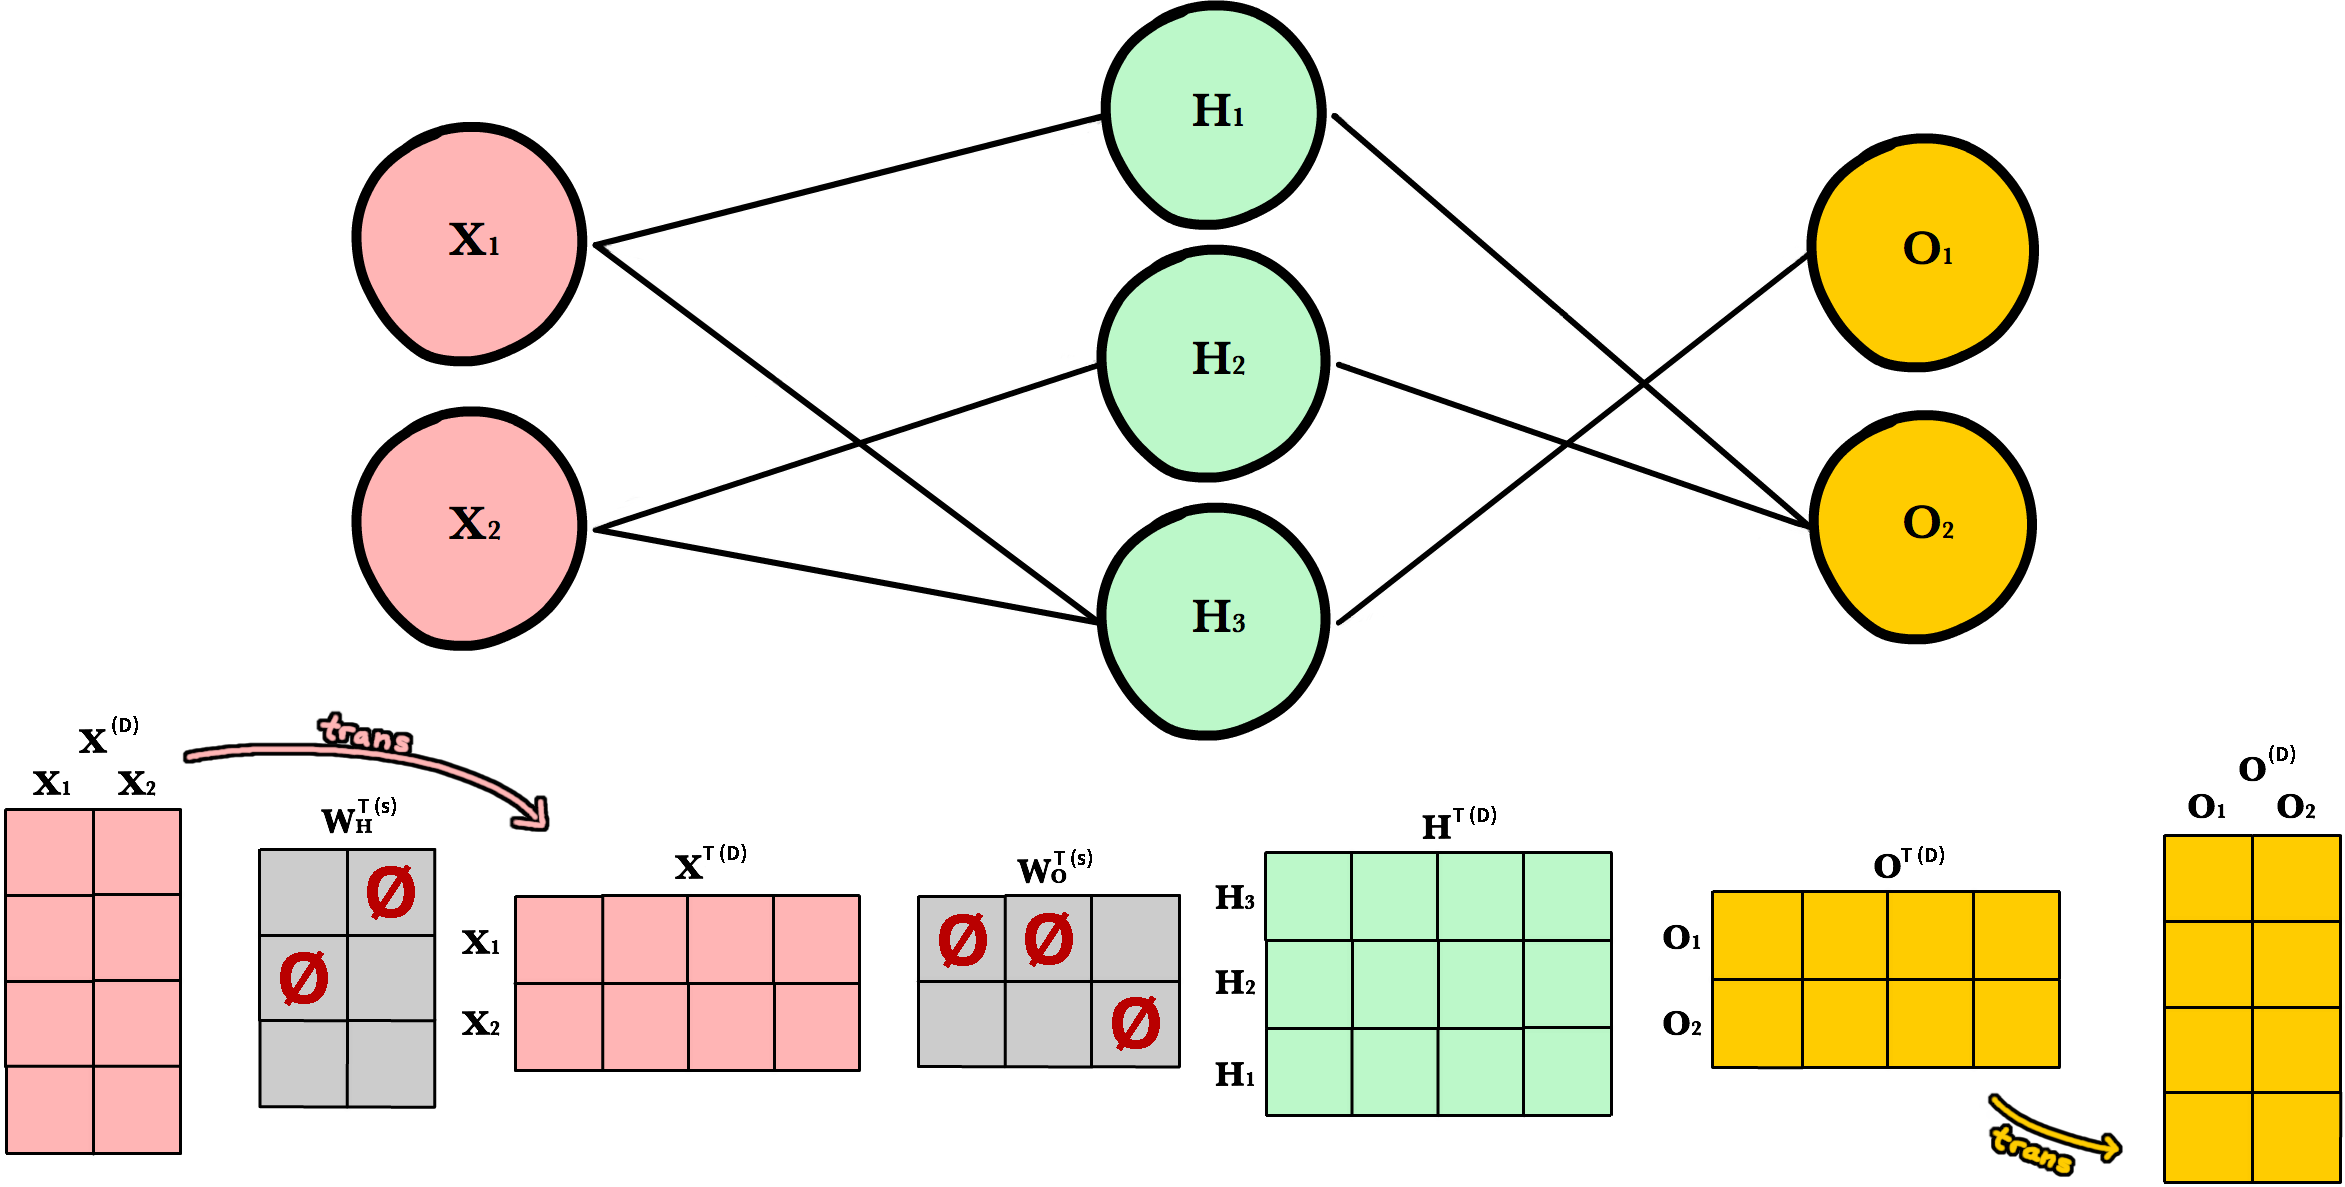
\includegraphics[width=\textwidth]{img/neural_network_matrix_sparse/neural_network_matrix_sparse.png}
    \caption{Visualización de inferencia en redes neuronales dispersas}
    \label{fig:nn_matrix_sparse}
\end{figure}

Sin embargo, empleando las propiedades de las matrices, es posible modificar el orden de las mismas, y así poder encajar cada matriz en la firma. Para esto se emplea una propiedad básica de las matrices, $C^{T} = (AB)^{T} = A^{T}B^{T}$. De esta forma, al transponer la matriz de pesos mediante el parámetro \texttt{transA}, y multiplicando esto por la salida de la capa anterior, obtendremos la salida $C^{T}$. Esto supone un pequeño overhead, al tener que transponer la entrada a la capa de entrada, así como la salida de la capa de salida. Sin embargo, dicho overhead puede ser mitigado en gran medida, en función de la arquitectura de la red, así como de la fuente de datos, que es probable que con pequeñas modificaciones pueda exportar los datos transpuestos previamente.

Esta estrategia se puede apreciar en la Figura \ref{fig:nn_matrix_sparse}, donde a diferencia de la Figura \ref{fig:nn_matrix_dense} se han transpuesto los pesos y las entradas, y se ha etiquetado correspondientemente mediante superíndices.
